\documentclass[doktyp=marbeit,fontsize=12pt,sprache=english,draft=true,hausschrift=true,fleqn]{TUBAFarbeiten}

% packages
\usepackage{amsmath}
\usepackage[ngerman]{babel}
\usepackage{blindtext}
\usepackage{caption}
\usepackage{calc}
\usepackage{cite}
\usepackage{enumitem}
\usepackage[T1]{fontenc}
\usepackage{floatrow} % rows of table and pictures
\usepackage{graphicx}
\usepackage{gensymb}
\usepackage[utf8]{inputenc}
\usepackage{makeidx}
\usepackage[fleqn]{mathtools} % mathtools und links buendig machen
\usepackage{subcaption}

% Images with mathcha.io 
\usepackage{tikz}
\usetikzlibrary{fadings}
\usepackage{mathdots}
\usepackage{yhmath}
\usepackage{cancel}
\usepackage{color}
\usepackage{siunitx}
\usepackage{array}
\usepackage{multirow}
\usepackage{amssymb}
\usepackage{gensymb}
\usepackage{tabularx}
\usepackage{booktabs}
% Images end

\usepackage{subscript} % tief stellen
%\usepackage[square]{natbib}
\usepackage{setspace}
\renewcommand{\baselinestretch}{1.5}

\usepackage{mathtools}
\DeclarePairedDelimiter{\ceil}{\lceil}{\rceil}
\DeclarePairedDelimiter{\floor}{\lfloor}{\rfloor}
\DeclarePairedDelimiter{\abs}{\lVert}{\rVert} % definiere absoluten betrag

\usepackage[acronym,toc]{glossaries}
\glstoctrue%

\newglossary[nlg]{symbols}{nls}{nlo}{Symbol Definition}
\makeglossaries%
\loadglsentries{glossary}
\loadglsentries{symbols}

% tubaf zeugs
\TUBAFFakultaet{Faculty of Mathematics and Computer Science}
\TUBAFInstitut{Institute for Computer Science}
\TUBAFLehrstuhl{Professorship for Virtual Reality and Multimedia}
\TUBAFTitel{Post-Processing of Depth Images and Laser Scan Data for Feature-based Pose Estimation}
\TUBAFBetreuer{Prof.\ Dr.\ Bernhard Jung}
\TUBAFKorrektor{M. Sc. Robert Lösch}
\TUBAFAutor[J. Toth]{Jonas Toth}
\TUBAFStudiengang{Master Angewandte Informatik}
\TUBAFMatrikel{57319}
% \TUBAFAnmeldeDatum[2019-09-25]{25. September 2019}
\TUBAFDatum{10. June 2020}


\setcounter{tocdepth}{3}
%\setcounter{secnumdepth}{3}

% \makeindex

% start the content
\begin{document}

\maketitle

\TUBAFErklaerungsseite%
\tableofcontents
\newpage

\printglossary[type=\acronymtype]%
\newpage

\printglossary[type=symbols]%
\glsaddallunused[symbols]
\newpage

\section{Introduction}

\subsection{Reasons for Importance}
\begin{itemize}
    \item multiple sensors per sensors
    \item depth sensors increasingly used in the field
    \item not-multimodal, laserscan can not be used / hardly used
    \item global positioning not easily done, because of local maxima and computational cost of for example particle based approaches
    \item performance/compute costs of ICP high
\end{itemize}

\subsection{Current State-of-the-Art}
\begin{itemize}
    \item registering depth and range data
    \item state of the art is ICP and variants, working point based or point to plane (TODO: cite ICP comparison paper)
    \item requires pointclouds of similar resolutions
    \item dependent on initial pose
\end{itemize}

\subsection{Other Approach}

\begin{itemize}
    \item Scaramuzza\cite{Scaramuzza2007} presented work on registering a camera to a laserscaner using manually selected features in the laserscan and the image
    \item prior conversion of the laserscan to an image dubbed \Glspl{bearing-angle-image}
    \item converted image shows the local geometric structure exposed to the scan

    \item Lin et.al \cite{Lin2017} applied SURF feature detection on \Glspl{bearing-angle-image}
    \item this allows feature based posed estimation with the classical workflow used in SLAM algorithms
\end{itemize}

\subsection{Improvements}

\begin{itemize}
    \item \Glspl{bearing-angle} is calculated in only one direction and can therefore not be rotation invariant
    \item this work proposes \Glspl{flexion-image} that encodes the local geometry in all directions and is rotation invariant
    \item multiple state-of-the-art keypoint detectors and feature descriptors are compared between \Glspl{flexion-image} and \Glspl{bearing-angle-image} on various datasets taken with Kinect v2 and a full Laserscan
    \item evaluation shows better performance of \Glspl{flexion-image} with regard to keypoint quality and feature description
\end{itemize}

\subsection{Structure of this Thesis}

\section{Related Work}

\subsection{Bearing-Angle and SURF}
Erratum for Scaramuzza and Lin
\subsection{Other Registrations (ICP)}
\subsection{Multi-Modal Sensor Registration}

\section{Fundamentals}

\subsection{Depth Sensors}
\subsubsection{Time-of-Flight}
\subsubsection{Structured Light}
\subsubsection{Laserscanner}

\subsection{Image formation and camera models}

\subsection{Keypoint Detection and Feature Description}
\subsection{Statistic of Binary Classifier}
\subsection{Edge-Preserving Filtering}

\section{Feature Images}

\subsection{Bearing-Angle}
\subsection{Flexion-Image}
\subsection{Discarded Approaches}
\subsubsection{Curvature}
\subsubsection{Multi-Directional Bearing Angle}

Formulas pictures and short computational evaluation.
Discussion of characteristic for Bearing Flexion.

\section{Experiments}

\subsection{Datasets}
\subsubsection{Synthetic Scene}
Blender with known trajectory?
\subsubsection{Lehrpfad Kinect}
\subsubsection{Office Kinect}
\subsubsection{Laserscans of Reiche Zeche, Wilhelm Süd}
\subsubsection{Laserscan transformed to pinhole}

\subsection{Implementation of Algorithms}
\subsection{Groundtruth Poses}
\subsection{Classification Evaluation}
\subsubsection{Approach with Backprojection and Distance Threshold}
\subsubsection{Statistical Kennziffern, what was looked at}
(Descriptors, Keypoints, Distribution, Size, Response)
\subsection{Algorithm Parameters}
\subsection{With insights, do another experiment with tuned parameters}
\subsection{Odometry with SLAM?!}

\section{Results}
\subsection{Show plain results and discuss outcome}

\section{Conclusion}

Very Sensors dependent, Time-of-flight and Laserscan gives the best quality.
SURF does not perform well, Bearing Angle gives lower response and less stability
Flexion is very nice.
FAST based stuff does not perform well, more exotic descriptors neither.
SIFT best, AKAZE very good.
Approach to transform depth image first before processing further works and gives results.

\subsection{Future Work}

\begin{itemize}
    \item BoW
    \item Laserscan with Kinect
    \item Other form of Ransac, that considers the depth information
    \item Performance Optimization, conversion is embarassingly parallel and computed on GPU
\end{itemize}


\newpage
\newpage
\newpage

\section{Old Texts}
\subsection{Goals}

Goals are registering pointclouds

\begin{figure}[H]
    \tikzset{every picture/.style={line width=0.75pt}} %set default line width to 0.75pt        

\begin{tikzpicture}[x=0.75pt,y=0.75pt,yscale=-1,xscale=1]
%uncomment if require: \path (0,519.5); %set diagram left start at 0, and has height of 519.5

%Flowchart: Data [id:dp9599947060349776] 
\draw  [color={rgb, 255:red, 74; green, 144; blue, 226 }  ,draw opacity=1 ] (60.98,13) -- (203.9,13) -- (170.92,53) -- (28,53) -- cycle ;
%Flowchart: Data [id:dp6428232547076108] 
\draw  [color={rgb, 255:red, 65; green, 117; blue, 5 }  ,draw opacity=1 ] (253.42,13) -- (406.9,13) -- (371.48,53) -- (218,53) -- cycle ;
%Flowchart: Process [id:dp1608692692695335] 
\draw  [color={rgb, 255:red, 65; green, 117; blue, 5 }  ,draw opacity=1 ] (218,104) -- (406.9,104) -- (406.9,174) -- (218,174) -- cycle ;
%Flowchart: Process [id:dp33893985253847336] 
\draw  [color={rgb, 255:red, 74; green, 144; blue, 226 }  ,draw opacity=1 ] (28,105) -- (203.9,105) -- (203.9,175) -- (28,175) -- cycle ;
%Straight Lines [id:da04782712814893719] 
\draw [color={rgb, 255:red, 74; green, 144; blue, 226 }  ,draw opacity=1 ]   (104.9,52.95) -- (104.9,103.95) ;
\draw [shift={(104.9,105.95)}, rotate = 270] [color={rgb, 255:red, 74; green, 144; blue, 226 }  ,draw opacity=1 ][line width=0.75]    (10.93,-3.29) .. controls (6.95,-1.4) and (3.31,-0.3) .. (0,0) .. controls (3.31,0.3) and (6.95,1.4) .. (10.93,3.29)   ;

%Straight Lines [id:da7341299406677789] 
\draw [color={rgb, 255:red, 65; green, 117; blue, 5 }  ,draw opacity=1 ]   (310.9,52.95) -- (310.9,101.95) ;
\draw [shift={(310.9,103.95)}, rotate = 270] [color={rgb, 255:red, 65; green, 117; blue, 5 }  ,draw opacity=1 ][line width=0.75]    (10.93,-3.29) .. controls (6.95,-1.4) and (3.31,-0.3) .. (0,0) .. controls (3.31,0.3) and (6.95,1.4) .. (10.93,3.29)   ;

%Straight Lines [id:da8466739584512232] 
\draw [color={rgb, 255:red, 74; green, 144; blue, 226 }  ,draw opacity=1 ]   (105.75,175) -- (105.75,200.87) ;
\draw [shift={(105.75,202.87)}, rotate = 270] [color={rgb, 255:red, 74; green, 144; blue, 226 }  ,draw opacity=1 ][line width=0.75]    (10.93,-3.29) .. controls (6.95,-1.4) and (3.31,-0.3) .. (0,0) .. controls (3.31,0.3) and (6.95,1.4) .. (10.93,3.29)   ;

%Flowchart: Data [id:dp9829119198657832] 
\draw  [color={rgb, 255:red, 74; green, 144; blue, 226 }  ,draw opacity=1 ] (60.98,203.55) -- (203.9,203.55) -- (170.92,243.55) -- (28,243.55) -- cycle ;
%Flowchart: Process [id:dp7985266301959889] 
\draw  [color={rgb, 255:red, 65; green, 117; blue, 5 }  ,draw opacity=1 ] (218,202.95) -- (406.9,202.95) -- (406.9,243.95) -- (218,243.95) -- cycle ;
%Flowchart: Merge [id:dp5897490340352475] 
\draw  [color={rgb, 255:red, 65; green, 117; blue, 5 }  ,draw opacity=1 ] (137.5,335.5) -- (284.5,335.5) -- (211,406.95) -- cycle ;
%Curve Lines [id:da7376618706424286] 
\draw [color={rgb, 255:red, 65; green, 117; blue, 5 }  ,draw opacity=1 ]   (105.78,244.87) .. controls (105.78,312.19) and (193.96,282.56) .. (196.69,333.38) ;
\draw [shift={(196.75,334.95)}, rotate = 268.92] [color={rgb, 255:red, 65; green, 117; blue, 5 }  ,draw opacity=1 ][line width=0.75]    (10.93,-3.29) .. controls (6.95,-1.4) and (3.31,-0.3) .. (0,0) .. controls (3.31,0.3) and (6.95,1.4) .. (10.93,3.29)   ;

%Curve Lines [id:da031417808526526425] 
\draw [color={rgb, 255:red, 65; green, 117; blue, 5 }  ,draw opacity=1 ]   (310.78,244.87) .. controls (310.78,281.31) and (242.84,297.46) .. (240.8,333.3) ;
\draw [shift={(240.75,334.95)}, rotate = 270] [color={rgb, 255:red, 65; green, 117; blue, 5 }  ,draw opacity=1 ][line width=0.75]    (10.93,-3.29) .. controls (6.95,-1.4) and (3.31,-0.3) .. (0,0) .. controls (3.31,0.3) and (6.95,1.4) .. (10.93,3.29)   ;

%Flowchart: Process [id:dp6519384117074126] 
\draw  [color={rgb, 255:red, 65; green, 117; blue, 5 }  ,draw opacity=1 ] (130.75,442.15) -- (294.75,442.15) -- (294.75,493.15) -- (130.75,493.15) -- cycle ;
%Straight Lines [id:da11178033003390464] 
\draw [color={rgb, 255:red, 65; green, 117; blue, 5 }  ,draw opacity=1 ]   (211,406.95) -- (211,441.3) ;
\draw [shift={(211,443.3)}, rotate = 270] [color={rgb, 255:red, 65; green, 117; blue, 5 }  ,draw opacity=1 ][line width=0.75]    (10.93,-3.29) .. controls (6.95,-1.4) and (3.31,-0.3) .. (0,0) .. controls (3.31,0.3) and (6.95,1.4) .. (10.93,3.29)   ;

%Straight Lines [id:da5794219109061295] 
\draw [color={rgb, 255:red, 74; green, 144; blue, 226 }  ,draw opacity=1 ]   (422,25) -- (442.75,25) ;


%Straight Lines [id:da9483137381576471] 
\draw [color={rgb, 255:red, 65; green, 117; blue, 5 }  ,draw opacity=1 ]   (422,54) -- (442.75,54) ;


%Straight Lines [id:da6404550524489918] 
\draw [color={rgb, 255:red, 65; green, 117; blue, 5 }  ,draw opacity=1 ]   (310.78,174.87) -- (310.78,200.87) ;
\draw [shift={(310.78,202.87)}, rotate = 270] [color={rgb, 255:red, 65; green, 117; blue, 5 }  ,draw opacity=1 ][line width=0.75]    (10.93,-3.29) .. controls (6.95,-1.4) and (3.31,-0.3) .. (0,0) .. controls (3.31,0.3) and (6.95,1.4) .. (10.93,3.29)   ;


% Text Node
\draw (120.95,33) node [color={rgb, 255:red, 74; green, 144; blue, 226 }  ,opacity=1 ] [align=left] {reference data\\pointclouds};
% Text Node
\draw (312.45,33) node [color={rgb, 255:red, 65; green, 117; blue, 5 }  ,opacity=1 ] [align=left] {sensor data\\depth images};
% Text Node
\draw (312.45,139) node [color={rgb, 255:red, 65; green, 117; blue, 5 }  ,opacity=1 ] [align=left] {conversion to\\feature image};
% Text Node
\draw (115.95,140) node [color={rgb, 255:red, 74; green, 144; blue, 226 }  ,opacity=1 ] [align=left] {conversion to\\feature image};
% Text Node
\draw (115.95,223.55) node [color={rgb, 255:red, 74; green, 144; blue, 226 }  ,opacity=1 ] [align=left] {Bag-of-Words};
% Text Node
\draw (312.45,223.45) node [color={rgb, 255:red, 65; green, 117; blue, 5 }  ,opacity=1 ] [align=left] {Feature Detection};
% Text Node
\draw (212,357.5) node [color={rgb, 255:red, 65; green, 117; blue, 5 }  ,opacity=1 ] [align=left] {Feature\\Matching};
% Text Node
\draw (218,467.65) node [color={rgb, 255:red, 65; green, 117; blue, 5 }  ,opacity=1 ] [align=left] {Pose Estimation};
% Text Node
\draw (527,24) node [color={rgb, 255:red, 74; green, 144; blue, 226 }  ,opacity=1 ] [align=left] {Offline Preprocessing};
% Text Node
\draw (516.5,53) node [color={rgb, 255:red, 65; green, 117; blue, 5 }  ,opacity=1 ] [align=left] {Online Processing};
% Text Node
\draw (140.9,78) node [scale=0.8] [align=left] {{\footnotesize \textcolor[rgb]{0.29,0.56,0.89}{Keyframes as}}\\{\footnotesize \textcolor[rgb]{0.29,0.56,0.89}{Cubemap}}\\{\footnotesize \textcolor[rgb]{0.29,0.56,0.89}{Images}}};
% Text Node
\draw (346,76) node [scale=0.8,color={rgb, 255:red, 126; green, 211; blue, 33 }  ,opacity=1 ] [align=left] {{\footnotesize \textcolor[rgb]{0.25,0.46,0.02}{Pinhole}}\\{\footnotesize \textcolor[rgb]{0.25,0.46,0.02}{Intrinsic}}};
% Text Node
\draw (218,285.4) node [scale=0.8] [align=left] {SIFT\\SURF\\AKAZE\\ORB};


\end{tikzpicture}

	\caption[Flowchart of final processing pipeline]{The final processing pipeline is able to register depth images in existing pointclouds with much higher resolution}
\end{figure}

\begin{figure}[H]
    \centering
    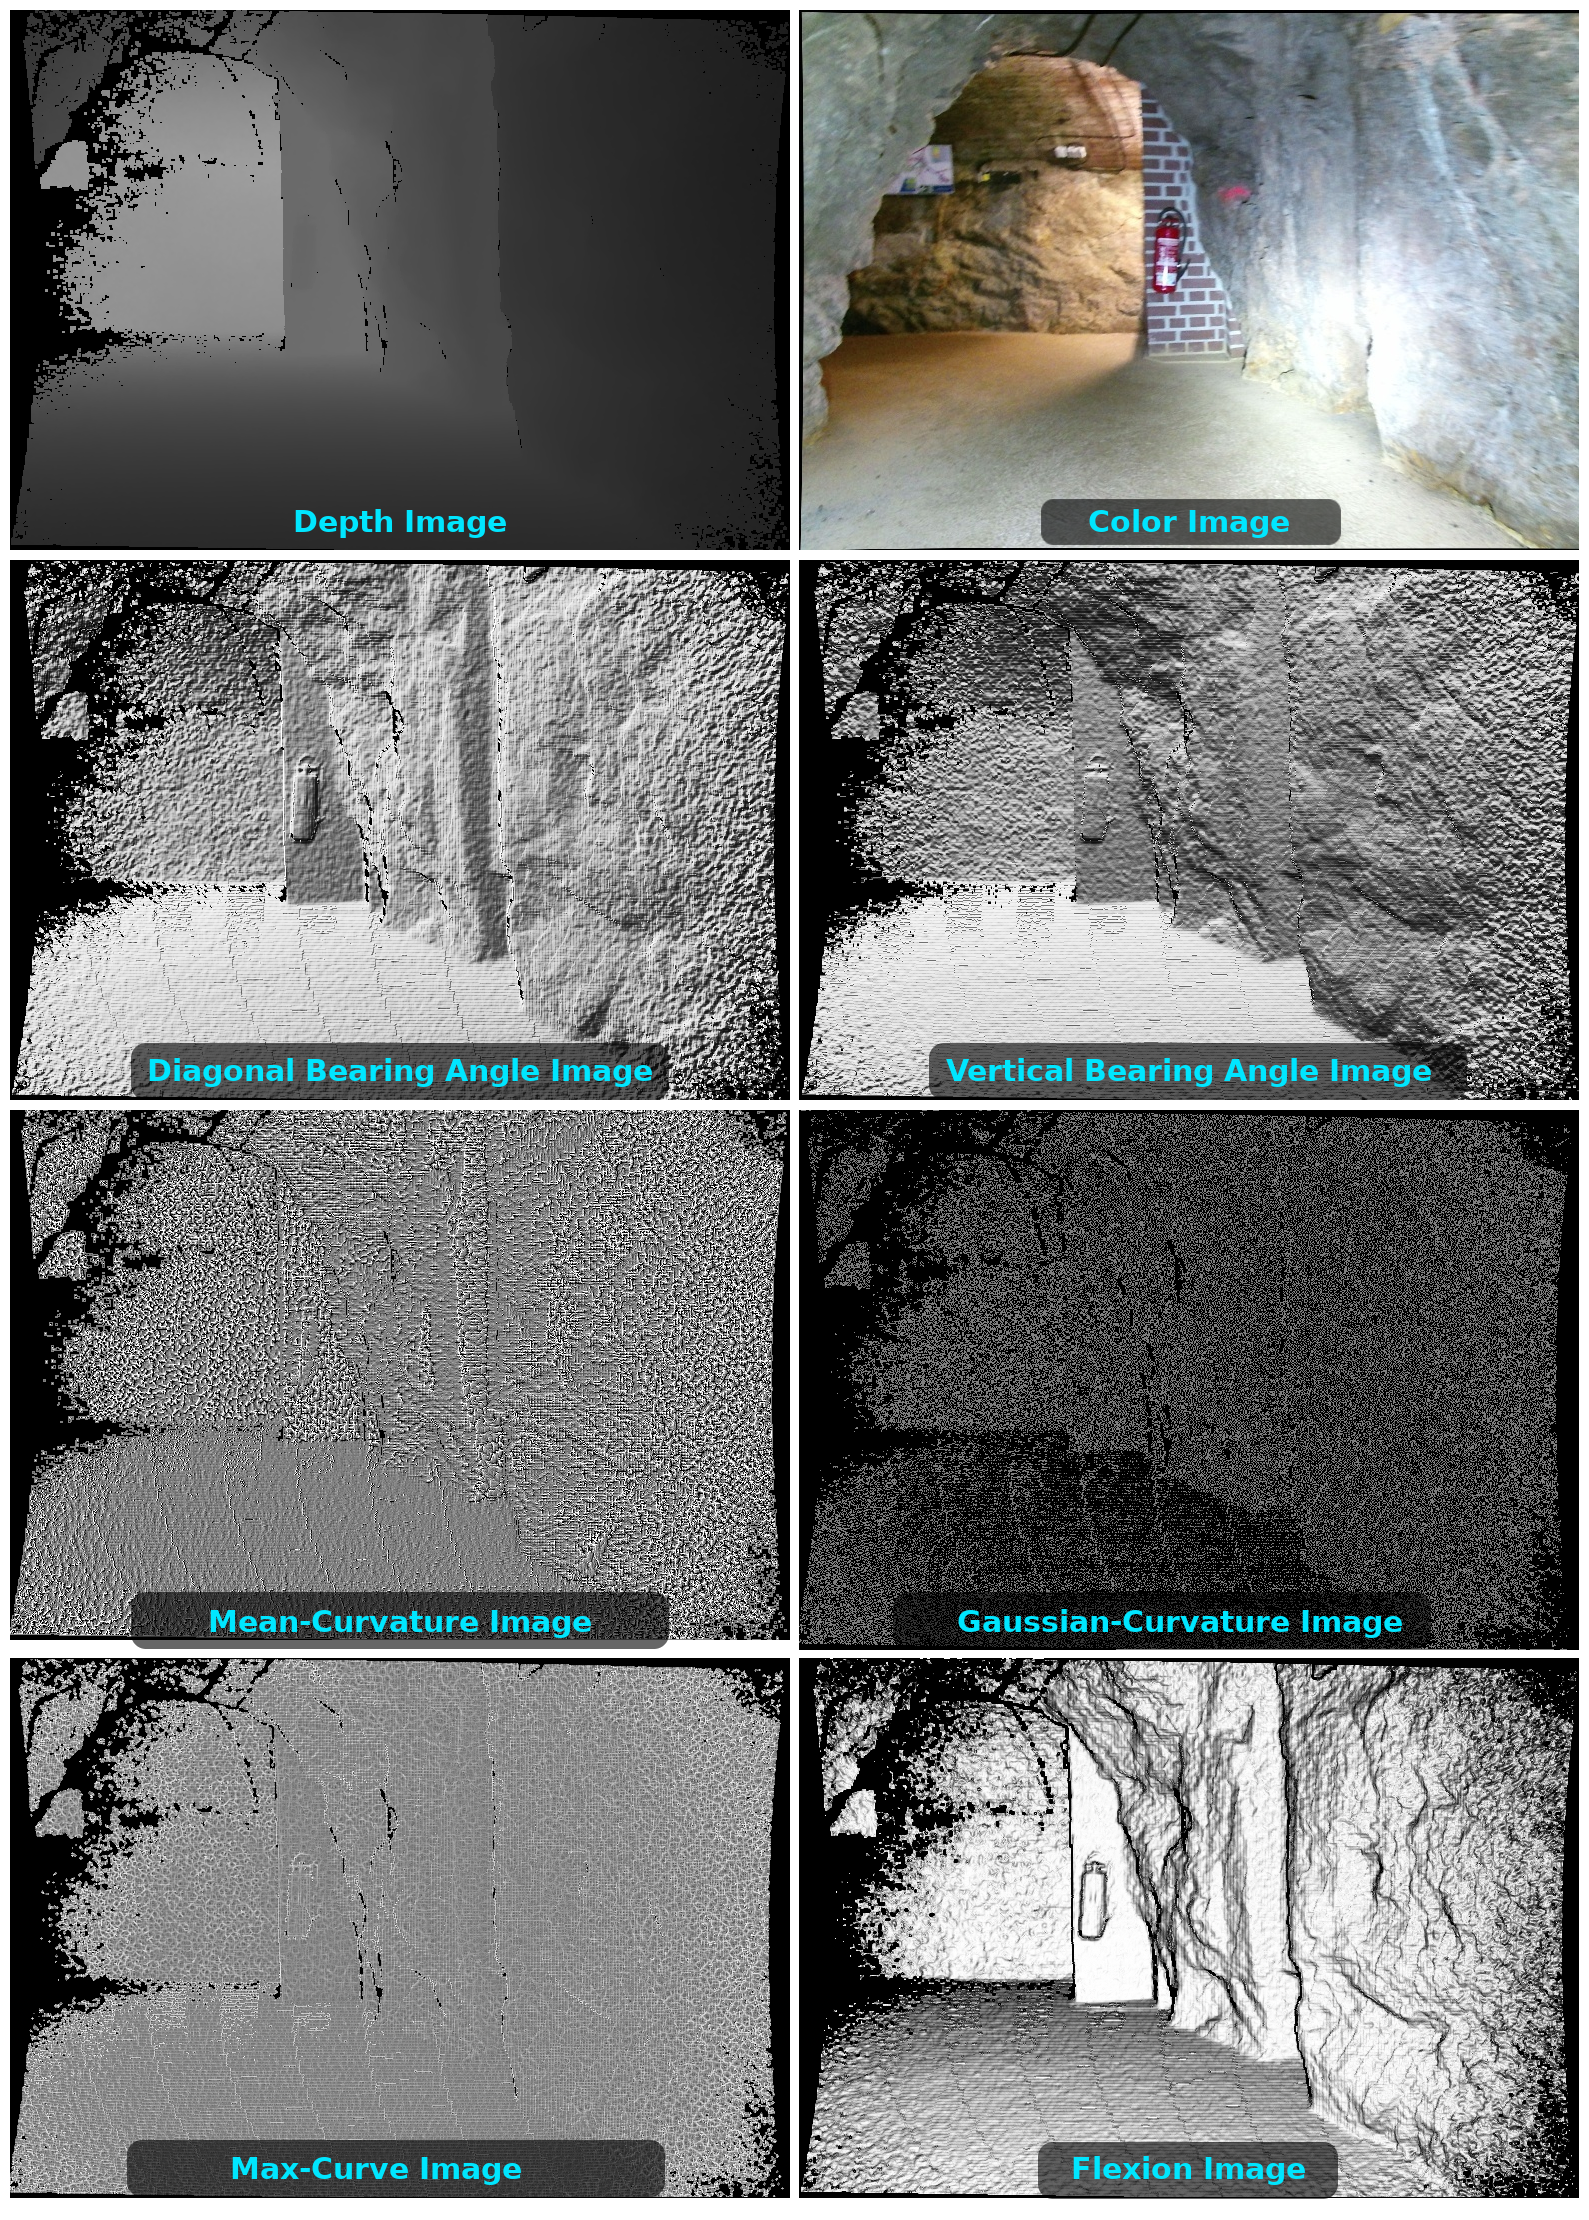
\includegraphics[width=0.9\textwidth]{images/collage_v3.png}
    \caption{Overview of possible Feature-Images from a depth image.}
\end{figure}

\subsection{Reference Data Processing}

\begin{figure}[H]
	\includegraphics[width=\linewidth]{images/bild1.png}
	\caption[Laserscan as equirectangular depth image]{This image shows a laserscan that is converted into an equirectangular depth image}
\end{figure}

\subsection{Feature Matching}

\begin{figure}[H]
	\includegraphics[width=\linewidth]{images/match-result.png}
	\caption[Examplaric Image Matching]{Matching two flexion images is possible, the results are mixed though. This match is done with ORB}
\end{figure}

\subsection{Potential Deviations from Plan}

\subsubsection*{Feature Matching Considerations}
\begin{itemize}
    \item depth-map preprocessing to fill holes and improve their quality
    \item smoothing or either depth-maps or feature images
    \item pyramid approach for multi-resolution feature images (similar to SIFT)
    \item change offset of neighbour pixels (e.g.~four pixel difference in each direction instead of just one)
    \item concentrate more on deep and wide evaluation of feature matching instead of full localization pipeline as a more robust foundation for future work
    \item just try out an out-of-the-box SfM-solution
\end{itemize}


\section{Introduction}

The dominant method to register pointclouds with pointclouds or depth
images is the use of a variant of the \gls{icp}\cite{Besl1992}
algorithm. Pomerleau et.al\cite{Pomerleau2015} provide a review of pointcloud registration methods.
Even though there are many different variations of \gls{icp}, it has
some common problems. The algorithm requires a good initial
transformation. Pointclouds with order-of-magnitude different
resolutions can produce unstable results. Convergence might require many
iterative steps and can not be predicted. Each of these iterative steps
is computationally expensive and does not scale very well to massive
datasets.

All these apsects give opportunity for a better solution to the problem
of registering depth images, e.g.~from the Kinect-v2, to existing
high-resolution pointclouds.
Inspired by Scaramuzza's \Glspl{bearing-angle-image}\cite{Scaramuzza2007}, Lin et.al\cite{Lin2017} apply the classical feature detector \gls{surf}\cite{Bay2006} on \Glspl{bearing-angle-image} and are able to register pointclouds to each other.
This work improves upon this idea in multiple ways.
\Glspl{bearing-angle-image} are not rotation invariant as they encode local geometry only in one direction.
Neither are they viewpoint invariant, as the \gls{bearing-angle} changes when the sensing lightray hits the same surface from a different angle.
In an attempt to overcome these limitations this work proposes new derived images that are rotation and viewpoint invariant, with the most promising variant being \Glspl{flexion-image}.

\section{Approach}\label{approach}

\subsection{Sensor description}

\begin{itemize}
    \item Determine Angular resolution for two light-rays, Laserscans are known and image sensors require intrinsic
    \item for Kinect, simplified pinhole model without distortion is assumed, rectification can be done beforehand
    \item resulting pictures are depth maps, that need conversion to euclidian distances
    \item Depth-Maps need to be converted into range data
\end{itemize}

\begin{figure}[H]
    \tikzset{every picture/.style={line width=0.75pt}} %set default line width to 0.75pt        

\begin{tikzpicture}[x=0.75pt,y=0.75pt,yscale=-1,xscale=1]
%uncomment if require: \path (0,300); %set diagram left start at 0, and has height of 300

%Straight Lines [id:da4352835258494677] 
\draw [color={rgb, 255:red, 74; green, 144; blue, 226 }  ,draw opacity=1 ][line width=2.25]    (173.83,252) -- (376.83,252) ;


%Flowchart: Connector [id:dp7899195950713407] 
\draw  [fill={rgb, 255:red, 0; green, 0; blue, 0 }  ,fill opacity=1 ] (326,252) .. controls (326,249.81) and (327.77,248.04) .. (329.96,248.04) .. controls (332.14,248.04) and (333.92,249.81) .. (333.92,252) .. controls (333.92,254.19) and (332.14,255.96) .. (329.96,255.96) .. controls (327.77,255.96) and (326,254.19) .. (326,252) -- cycle ;
%Flowchart: Connector [id:dp5223576666610675] 
\draw  [fill={rgb, 255:red, 0; green, 0; blue, 0 }  ,fill opacity=1 ] (223,50) .. controls (223,47.81) and (224.77,46.04) .. (226.96,46.04) .. controls (229.14,46.04) and (230.92,47.81) .. (230.92,50) .. controls (230.92,52.19) and (229.14,53.96) .. (226.96,53.96) .. controls (224.77,53.96) and (223,52.19) .. (223,50) -- cycle ;
%Straight Lines [id:da7852815672316228] 
\draw    (226.96,50) -- (226.96,252) ;


%Straight Lines [id:da3653242786315575] 
\draw    (226.96,50) -- (329.96,252) ;



% Text Node
\draw (251,271) node  [align=left] {Image Plane};
% Text Node
\draw (330,271) node  [align=left] {C};
% Text Node
\draw (215.96,157) node [rotate=-90] [align=left] {orthographic depth};
% Text Node
\draw (287,135) node [rotate=-63.14] [align=left] {euclidian depth};

\end{tikzpicture}

    \caption[Range Data and Depth Maps visualized]{Depthimages encode the othorgraphic depth. For the following calculations the conversion to the euclidian depth is necessary as first preprocessing step.}
\end{figure}

Projecting pixels onto the unit sphere.
\begin{align}
	\begin{pmatrix}x \\ y \\ z \end{pmatrix} &= \begin{pmatrix} \frac{u - c_x}{f_x} \\ \frac{v - c_y}{f_y} \\ 1 \end{pmatrix} \\
	\begin{pmatrix}x_s \\ y_s \\ z_s \end{pmatrix} &= \frac{\sqrt{1 + x^2 + y^2}}{1 + x^2 + y^2} \begin{pmatrix} x \\ y \\ z \end{pmatrix}
\end{align}

\begin{itemize}
    \item Angular resolution between two pixels needs to be calculated for the camera
    \item intrinsic calibration required, but can be cached statically afterwards
\end{itemize}

\begin{figure}[H]
    

\tikzset{every picture/.style={line width=0.75pt}} %set default line width to 0.75pt        

\begin{tikzpicture}[x=0.75pt,y=0.75pt,yscale=-1,xscale=1]
%uncomment if require: \path (0,300); %set diagram left start at 0, and has height of 300

%Shape: Circle [id:dp9330703578589419] 
\draw   (21.58,147.92) .. controls (21.58,67.33) and (86.91,2) .. (167.5,2) .. controls (248.09,2) and (313.42,67.33) .. (313.42,147.92) .. controls (313.42,228.5) and (248.09,293.83) .. (167.5,293.83) .. controls (86.91,293.83) and (21.58,228.5) .. (21.58,147.92) -- cycle ;
%Shape: Circle [id:dp9657721103702154] 
\draw  [fill={rgb, 255:red, 0; green, 0; blue, 0 }  ,fill opacity=1 ] (163.08,147.92) .. controls (163.08,145.48) and (165.06,143.5) .. (167.5,143.5) .. controls (169.94,143.5) and (171.92,145.48) .. (171.92,147.92) .. controls (171.92,150.36) and (169.94,152.33) .. (167.5,152.33) .. controls (165.06,152.33) and (163.08,150.36) .. (163.08,147.92) -- cycle ;
%Shape: Circle [id:dp5918706400105579] 
\draw  [fill={rgb, 255:red, 0; green, 0; blue, 0 }  ,fill opacity=1 ] (262.08,71.92) .. controls (262.08,69.48) and (264.06,67.5) .. (266.5,67.5) .. controls (268.94,67.5) and (270.92,69.48) .. (270.92,71.92) .. controls (270.92,74.36) and (268.94,76.33) .. (266.5,76.33) .. controls (264.06,76.33) and (262.08,74.36) .. (262.08,71.92) -- cycle ;
%Shape: Ellipse [id:dp7276506054694092] 
\draw  [color={rgb, 255:red, 155; green, 155; blue, 155 }  ,draw opacity=1 ][dash pattern={on 4.5pt off 4.5pt}] (21.58,147.92) .. controls (21.58,123.89) and (86.91,104.42) .. (167.5,104.42) .. controls (248.09,104.42) and (313.42,123.89) .. (313.42,147.92) .. controls (313.42,171.94) and (248.09,191.42) .. (167.5,191.42) .. controls (86.91,191.42) and (21.58,171.94) .. (21.58,147.92) -- cycle ;
%Shape: Circle [id:dp534532540383378] 
\draw  [fill={rgb, 255:red, 0; green, 0; blue, 0 }  ,fill opacity=1 ] (292.08,117.92) .. controls (292.08,115.48) and (294.06,113.5) .. (296.5,113.5) .. controls (298.94,113.5) and (300.92,115.48) .. (300.92,117.92) .. controls (300.92,120.36) and (298.94,122.33) .. (296.5,122.33) .. controls (294.06,122.33) and (292.08,120.36) .. (292.08,117.92) -- cycle ;
%Straight Lines [id:da5608352336717536] 
\draw    (167.5,147.92) -- (266.5,71.92) ;


%Straight Lines [id:da5901973594450144] 
\draw    (167.5,147.92) -- (296.5,117.92) ;


%Shape: Arc [id:dp17654467766402726] 
\draw  [draw opacity=0] (233.41,97.68) .. controls (242.7,102.78) and (249,112.66) .. (249,124) .. controls (249,125.96) and (248.81,127.88) .. (248.45,129.74) -- (219,124) -- cycle ; \draw  [color={rgb, 255:red, 208; green, 2; blue, 27 }  ,draw opacity=1 ] (233.41,97.68) .. controls (242.7,102.78) and (249,112.66) .. (249,124) .. controls (249,125.96) and (248.81,127.88) .. (248.45,129.74) ;

% Text Node
\draw (225,120) node [color={rgb, 255:red, 208; green, 2; blue, 27 }  ,opacity=1 ] [align=left] {$\displaystyle \Delta \varphi $};
% Text Node
\draw (167,165) node  [align=left] {C};


\end{tikzpicture}


	\caption[Angle between two pixels in the pinhole model]{The angle between two pixels of a rectified pinhole image.}
\end{figure}
To determine the angle spanned between two corresponding lightrays for two pixels the pixel coordinate needs to be backprojected to the unit sphere.
\begin{align}
    \begin{pmatrix} u \\ v \end{pmatrix} \mapsto \begin{pmatrix} x_s \\ y_s \\ z_s \end{pmatrix}
\end{align}
The resulting vectors have unit length, simplifying the angle-calculation.
\begin{align}
    \vec{r_1} \cdot \vec{r_2} &= \abs{\vec{r_1}} \abs{\vec{r_2}} \cos \Delta\varphi \\
    \cos \Delta\varphi &= x_{s,1} x_{s,2} + y_{s,1} y_{s,2} + z_{s,1} z_{s,2} \\
    \Delta\varphi &= \arccos{x_{s,1} x_{s,2} + y_{s,1} y_{s,2} + z_{s,1} z_{s,2}}
\end{align}
The angle $\Delta\varphi$ is not a constant for the pinhole model for different pixels but can be calculated once for each intrinsic.

\subsection{Preprocessing of range Data}\label{preprocessing-of-range-data}

\begin{figure}[H]
    \centering
    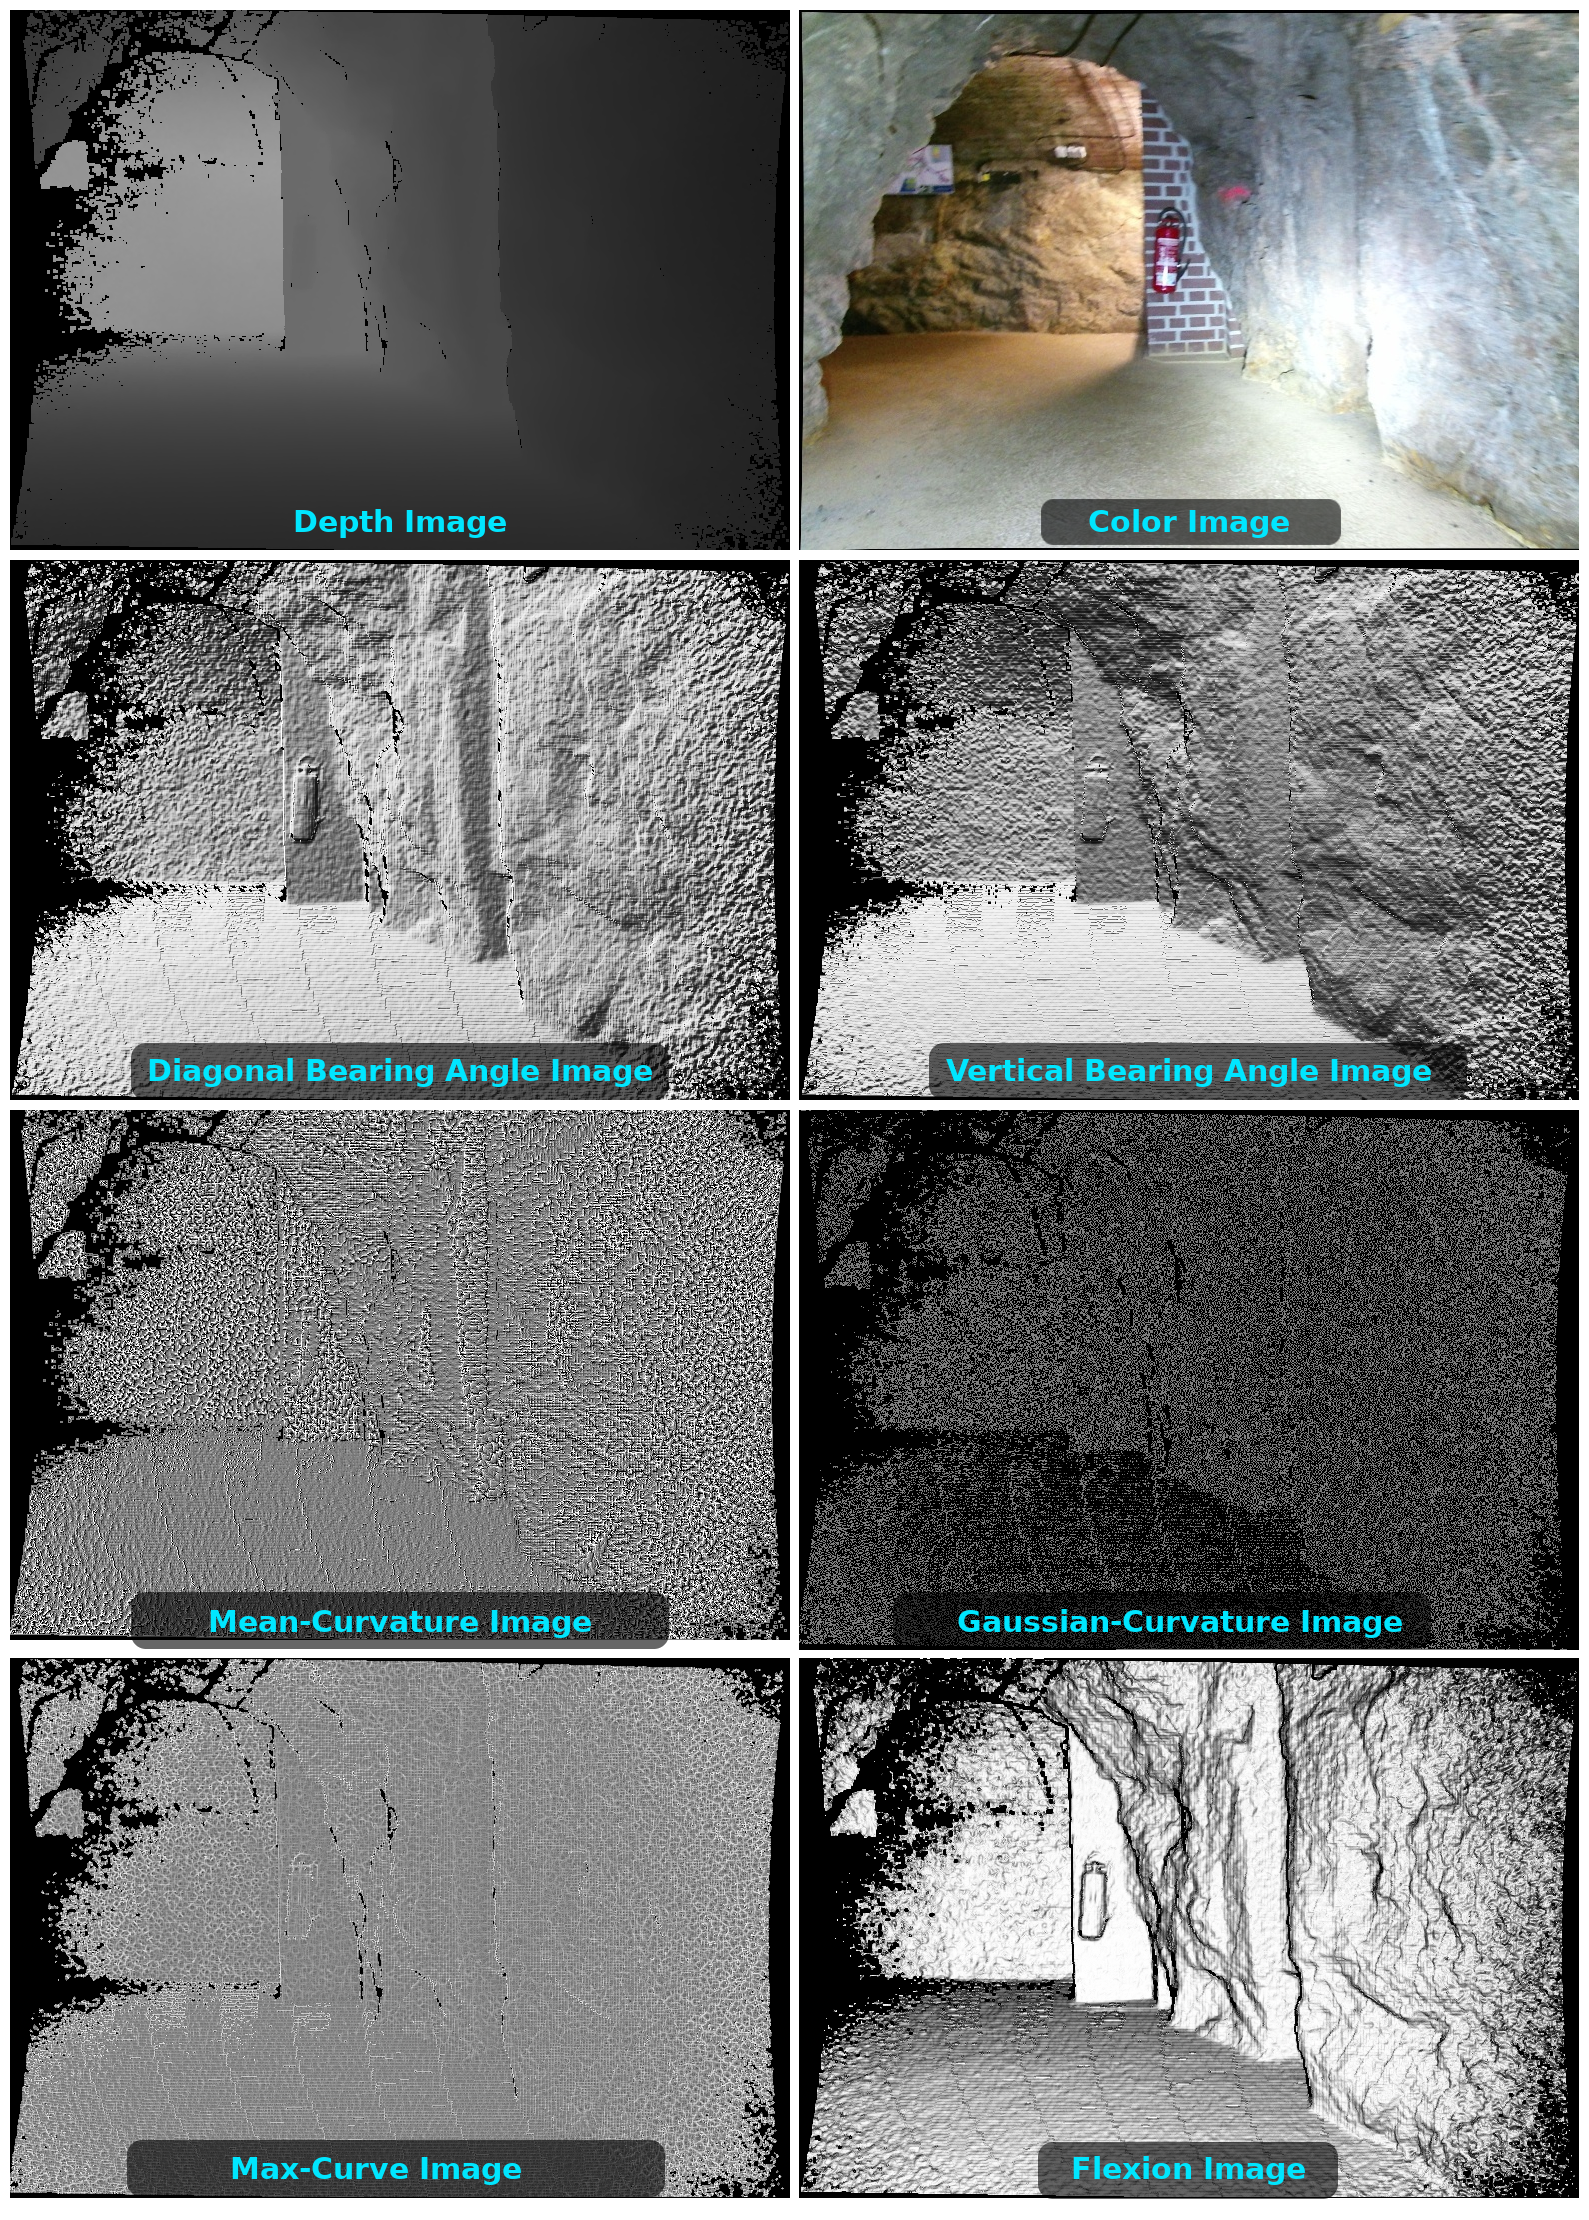
\includegraphics[width=0.9\textwidth]{images/collage_v3.png}
    \caption{Overview of possible Feature-Images from a depth image.}
\end{figure}

Instead of registering the depth images based on single points as \gls{icp} algorithms do, this thesis develops a new framework to use existing image features like \Gls{sift} and \Gls{surf} to calculate the transformation between pointcloud and depth image.
Both, the pointcloud and the depth image, are first converted to a gray-scale feature image.
Local geometric structure is encoded through the visual structure of the feature image and is detected and matched via a classical matching pipeline.

In general depth images do not contain a valid value for each pixel.
The Kinectv2 returns $0$ if no measurement was possible.
Whenever such a value would be included in the calculation of the derived quantities the value is set to $0$ as well.

Each feature quantity has a different range of valid values.
To create visually distinct images these values are scaled and quantized to the image depth.
With $p$ the final value for the pixel, $t_{min}$ and $t_{max}$ the value range for the target image depth and $v$ the scalar value of the feature quantity, the conversion is done with the following formula.
\begin{align}
    p = \floor[\Bigg]{\frac{{(t_{max} - t_{min})} {(v - t_{min})}}{t_{max} - t_{min}} + t_{min}}
\end{align}
Depth images themself are usually stored as $16~bit~unsigned$ grayscale images.
For feature images with the same image depth $t_{min} = 0$ and $t_{max} = 65535$

\subsection{\Glspl{bearing-angle-image}}

\begin{figure}[H]
    \centering
    \tikzset{every picture/.style={line width=0.75pt}} %set default line width to 0.75pt        

\begin{tikzpicture}[x=0.75pt,y=0.75pt,yscale=-1,xscale=1]
%uncomment if require: \path (0,227.75); %set diagram left start at 0, and has height of 227.75

%Straight Lines [id:da05017383740499093] 
\draw    (38.83,15.67) -- (141.83,202.67) ;


%Straight Lines [id:da6895513561877372] 
\draw    (201.83,46.67) -- (141.83,202.67) ;


%Curve Lines [id:da10253757735662583] 
\draw [color={rgb, 255:red, 0; green, 0; blue, 0 }  ,draw opacity=1 ]   (109,143) .. controls (115.83,127.67) and (153.83,120.67) .. (164.83,143.67) ;


%Straight Lines [id:da3851492122035306] 
\draw    (38.83,15.67) -- (201.83,46.67) ;


%Curve Lines [id:da7052636563383052] 
\draw [color={rgb, 255:red, 208; green, 2; blue, 27 }  ,draw opacity=1 ]   (162.83,39.17) .. controls (155.83,61.17) and (166.9,81.48) .. (186.9,85.48) ;


%Shape: Circle [id:dp08101382020617043] 
\draw  [fill={rgb, 255:red, 0; green, 0; blue, 0 }  ,fill opacity=1 ] (197.88,46.67) .. controls (197.88,44.49) and (199.65,42.72) .. (201.83,42.72) .. controls (204.01,42.72) and (205.78,44.49) .. (205.78,46.67) .. controls (205.78,48.85) and (204.01,50.62) .. (201.83,50.62) .. controls (199.65,50.62) and (197.88,48.85) .. (197.88,46.67) -- cycle ;
%Shape: Circle [id:dp7397482298206297] 
\draw  [fill={rgb, 255:red, 0; green, 0; blue, 0 }  ,fill opacity=1 ] (34.88,15.67) .. controls (34.88,13.49) and (36.65,11.72) .. (38.83,11.72) .. controls (41.01,11.72) and (42.78,13.49) .. (42.78,15.67) .. controls (42.78,17.85) and (41.01,19.62) .. (38.83,19.62) .. controls (36.65,19.62) and (34.88,17.85) .. (34.88,15.67) -- cycle ;


% Text Node
\draw (139,158) node [color={rgb, 255:red, 0; green, 0; blue, 0 }  ,opacity=1 ] [align=left] {$\displaystyle \Delta $$\displaystyle \varphi $};
% Text Node
\draw (181,58) node [color={rgb, 255:red, 208; green, 2; blue, 27 }  ,opacity=1 ] [align=left] {$\displaystyle \beta $};
% Text Node
\draw (191,117) node  [align=left] {$\displaystyle d_{i}$};
% Text Node
\draw (67,110) node  [align=left] {$\displaystyle d_{i-1}$};
% Text Node
\draw (217,47) node  [align=left] {$\displaystyle P_{i}$};
% Text Node
\draw (20,14) node  [align=left] {$\displaystyle P_{i-1}$};
% Text Node
\draw (142,215) node  [align=left] {$\displaystyle C$};


\end{tikzpicture}
%
    \caption[Schematic Representation of Bearing-Angles]{This figure shows the relationship of the light rays that form the \gls{bearing-angle}.}
\end{figure}

Existing literature\cite{Scaramuzza2007,Lin2017} proposes \Glspl{bearing-angle-image} were each pixel is the angle between the current point, the optical center and the previous point.
The neighbourhood relationship can be choosen arbitrarily resulting in four first-order \Glspl{bearing-angle-image}, horizontal, vertical, diagonal and antidiagonal.
The second variable is the direction the angle is calculted, e.g.~for horizontal images it can be calculated from left-to-right or right-to-left.
This does not exhibit new information, because the angle of the other direction is immediatly known from the fact that the sum of the angles is $180\degree$.
Nontheless, the direction must be defined to obtain stable visual features.

The formula for the \gls{bearing-angle} $\beta$ is derived with the cosine theorem.
For the horizontal left-to-right calculation the formula is as follows.
\begin{align}
    \beta&= \arccos%
            \frac{d_{i,j} - d_{i-1,j} \cos \Delta\varphi}%
                 {\sqrt{d_{i,j}^2 + d_{i-1,j}^2 - 2 d_{i,j} d_{i-1,j} \cos \Delta\varphi}}
\end{align}
Using a different direction or other neighbourhood relation the indices for the depth values need to be changed and a different angular resolution needs to be calculated.
The \Gls{bearing-angle} is in the range $(0, \pi)~rad$ and gets scaled accordingly.

\subsection{\Glspl{flexion-image}}\label{flexion-image-section}

Each pixel of a \Gls{flexion-image} is the dot-product of the local normal
calculated from horizontal and vertical neighbouring pixel with the
normal calculated with the diagonal neighbours.
Figure~\ref{fig:flexion-image-scetched} demonstrates the disparity of both normals for an arbitrary surface patch.
The normal calculated from the diagonal and vertical neighbouring vertices are drawn in blue and the normal calculated with the diagonals red.
Both normal-vectors are drawn with their origin in the central depth value.

\begin{figure}[H]
    \centering
    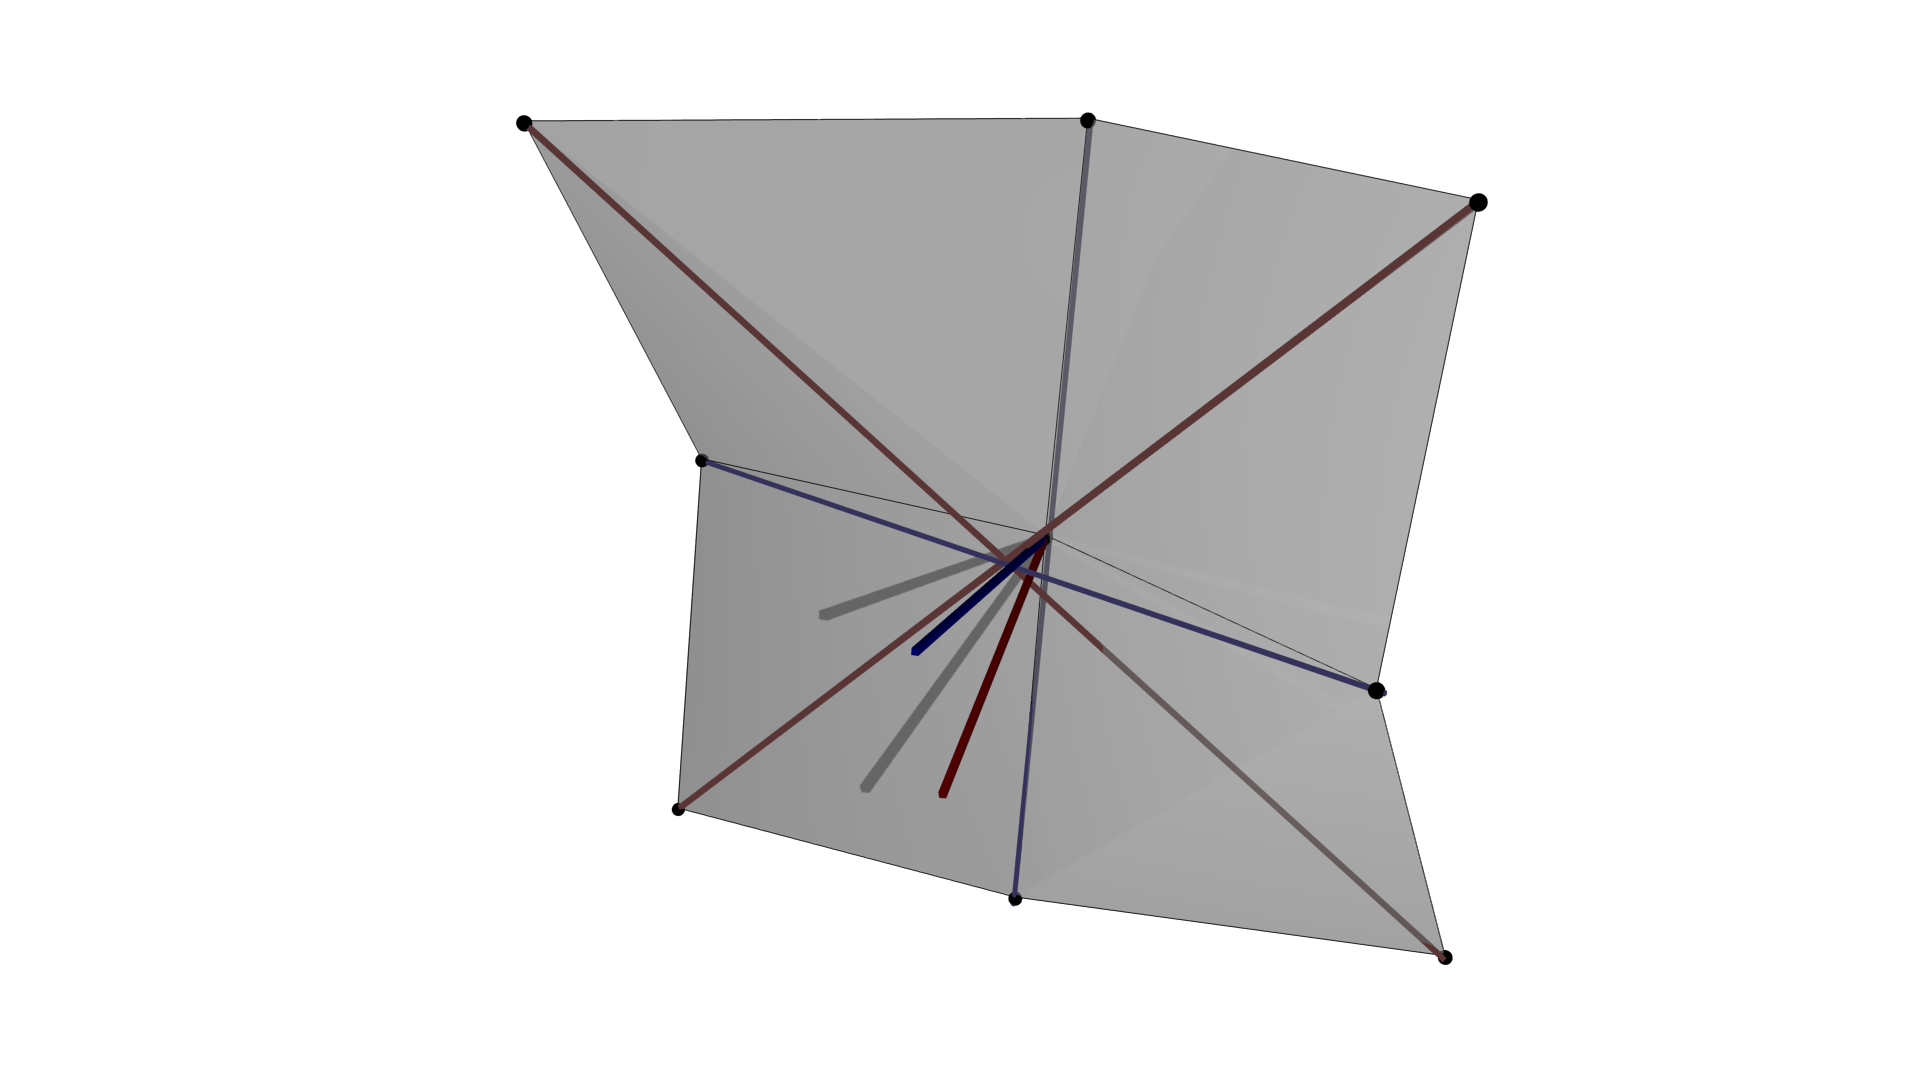
\includegraphics[width=0.6\textwidth]{images/scetch_flexion.png}
    \caption[Schematic Representation of Flexion]{This figure demonstrates how flexed surfaces have different normals for diagonal and non-diagonal estimation. This difference is utilized as measure for flexion.}%
    \label{fig:flexion-image-scetched}
\end{figure}

The flexion $f$ is defined as
\begin{align}
    f &= \abs{n_1 \cdotp n_2}
\end{align}
Because $n_1$ and $n_2$ are of length $1$ the value of $f$ is in the range $[0, 1]$ and gets scaled accordingly.

The smaller the dot-product gets, the higher is the local flexion of the
surface. This local property of the geometry then results in visual
features detectable with classical feature detectors and descriptors like
\Gls{sift} or \Gls{surf}.

\subsection{Other derived feature quantities}

Other attempts to create feature images are described in the thesis as well.
The performance in feature detection and matching is compared.
From visual inspection the author expects \Glspl{flexion-image} to perform best though.

The \gls{max-curve-image} tries generalize the \gls{bearing-angle} to be rotation invariant as it takes the \gls{bearing-angle} in each direction into account.
Additionally to the left-sided \gls{bearing-angle} the right-sided angle is calculated as well and finally added.

\begin{figure}
    \tikzset{every picture/.style={line width=0.75pt}} %set default line width to 0.75pt        

\begin{tikzpicture}[x=0.75pt,y=0.75pt,yscale=-1,xscale=1]
%uncomment if require: \path (0,252.25); %set diagram left start at 0, and has height of 252.25

%Straight Lines [id:da05017383740499093] 
\draw    (46.83,26.67) -- (149.83,213.67) ;


%Straight Lines [id:da6895513561877372] 
\draw    (155.83,32.67) -- (149.83,213.67) ;


%Curve Lines [id:da10253757735662583] 
\draw [color={rgb, 255:red, 0; green, 0; blue, 0 }  ,draw opacity=1 ]   (116,153) .. controls (128.83,126.67) and (169.83,125.67) .. (181.83,145.67) ;


%Straight Lines [id:da3851492122035306] 
\draw    (46.83,26.67) -- (155.83,32.67) ;


%Curve Lines [id:da7052636563383052] 
\draw [color={rgb, 255:red, 208; green, 2; blue, 27 }  ,draw opacity=1 ]   (118.83,30.67) .. controls (113.83,48.67) and (127.83,77.67) .. (154.83,77.67) ;


%Shape: Circle [id:dp08101382020617043] 
\draw  [fill={rgb, 255:red, 0; green, 0; blue, 0 }  ,fill opacity=1 ] (151.88,32.67) .. controls (151.88,30.49) and (153.65,28.72) .. (155.83,28.72) .. controls (158.01,28.72) and (159.78,30.49) .. (159.78,32.67) .. controls (159.78,34.85) and (158.01,36.62) .. (155.83,36.62) .. controls (153.65,36.62) and (151.88,34.85) .. (151.88,32.67) -- cycle ;
%Shape: Circle [id:dp7397482298206297] 
\draw  [fill={rgb, 255:red, 0; green, 0; blue, 0 }  ,fill opacity=1 ] (42.88,26.67) .. controls (42.88,24.49) and (44.65,22.72) .. (46.83,22.72) .. controls (49.01,22.72) and (50.78,24.49) .. (50.78,26.67) .. controls (50.78,28.85) and (49.01,30.62) .. (46.83,30.62) .. controls (44.65,30.62) and (42.88,28.85) .. (42.88,26.67) -- cycle ;
%Shape: Circle [id:dp7936487176657823] 
\draw  [fill={rgb, 255:red, 0; green, 0; blue, 0 }  ,fill opacity=1 ] (241.88,7.67) .. controls (241.88,5.49) and (243.65,3.72) .. (245.83,3.72) .. controls (248.01,3.72) and (249.78,5.49) .. (249.78,7.67) .. controls (249.78,9.85) and (248.01,11.62) .. (245.83,11.62) .. controls (243.65,11.62) and (241.88,9.85) .. (241.88,7.67) -- cycle ;
%Straight Lines [id:da7225304487809803] 
\draw    (245.83,7.67) -- (149.83,213.67) ;


%Straight Lines [id:da15289701870660388] 
\draw    (155.83,32.67) -- (245.83,7.67) ;


%Curve Lines [id:da9153553751002029] 
\draw [color={rgb, 255:red, 245; green, 166; blue, 35 }  ,draw opacity=1 ]   (154.83,77.67) .. controls (178.83,81.67) and (200.83,49.67) .. (184.83,24.67) ;



% Text Node
\draw (136,148) node [color={rgb, 255:red, 0; green, 0; blue, 0 }  ,opacity=1 ] [align=left] {$\displaystyle \Delta $$\displaystyle \varphi $};
% Text Node
\draw (142,48) node [color={rgb, 255:red, 208; green, 2; blue, 27 }  ,opacity=1 ] [align=left] {$\displaystyle \beta $};
% Text Node
\draw (167,100) node  [align=left] {$\displaystyle d_{i}$};
% Text Node
\draw (75,121) node  [align=left] {$\displaystyle d_{i-1}$};
% Text Node
\draw (153,12) node  [align=left] {$\displaystyle P_{i}$};
% Text Node
\draw (24,25) node  [align=left] {$\displaystyle P_{i-1}$};
% Text Node
\draw (150,226) node  [align=left] {$\displaystyle C$};
% Text Node
\draw (276,7) node  [align=left] {$\displaystyle P_{i+1}$};
% Text Node
\draw (229,108) node  [align=left] {$\displaystyle d_{i+1}$};
% Text Node
\draw (170,47) node  [align=left] {$\displaystyle \textcolor[rgb]{0.96,0.65,0.14}{\gamma }$};
% Text Node
\draw (166,149) node [color={rgb, 255:red, 0; green, 0; blue, 0 }  ,opacity=1 ] [align=left] {$\displaystyle \Delta $$\displaystyle \theta $};


\end{tikzpicture}

    \caption[Schematic Representation of the Max-Curve]{The Max-Curve composes two \Glspl{bearing-angle} in vertical, horizontal, diagonal and antidiagonal direction. The maximum angle is then selected as pixel value.}
\end{figure}

This makes the measure more robust to rotation, but does not produce good features.
\begin{align}
    B_{max} &= \max{\{B_{diagonal}, B_{antidiagonal}, B_{horizontal}, B_{vertical}\}}
\end{align}

As a different analytical approach to producing feature images the calculation of the \gls{curvature} for each depth value.
The two common measures of curvature in differential geometry are \gls{gaussian-curvature} and \gls{mean-curvature}\cite{Kuhnel2008}.

If the function is known as a graph the \Gls{gaussian-curvature} can be estimated using the derivatives of the function.
For depth data each depth value is a sample of this function graph and numeric approximation of the derivatives allows the calculation of the curvature.
\begin{align}
    \mathfrak{K} &= \frac{f_{uu} f_{vv} - f_{uv}^2}{{(1 + f_u^2 + f_v^2)}^2}
\end{align}
With
\begin{align*}
    f_{x} &= \frac{y_1 - y_0}{\Delta x} \\
    f_{xx} &= \frac{y_1 + y_{-1} - 2 y_0}{{\Delta x}^2}
\end{align*}
as approximation for the derivatives.

Similarly, the \Gls{mean-curvature} can be calculated with a different formula.
\begin{align}
    \mathfrak{H} &= \frac{{(1 + f_{v}^2)} f_{uu} - 2 f_u f_v f_{uv} + {(1 + f_u^2)} f_{vv}}{2 \sqrt{1 + f_u^2 + f_v^2}^3}
\end{align}
Both measures of curvature are $\mathfrak{K},\mathfrak{H} \in {\rm I\!R}$.
To convert them into a meaningful grayscale image they need to be clamped to arbitrary bounds, that can be choosen based on visual distinctiveness or other heuristics.
After clamping the values are scaled and quantized accordingly.

All of those experiments are implemented and compared in the thesis.

\subsection{Transformation calculation}\label{transformation-calculation}

Starting with the feature image, a visual localization pipeline is
established that works solely on omnidirectional data, thus is general
enough to utilize a wide range of sensors and camera models.

The full workflow of the pipeline is as follows:

\begin{enumerate}
\item Omnidirectional images are mapped onto a cubemap to reduce distortion,
  the feature images are calculated for both the data to localize,
  e.g.~Kinect depth image and the reference data, e.g.~terrestrial
  laserscans.
\item Visual Features are detected and matched between the sensor to
  localize and the reference data.
\item Classical RANSAC performs the stable calculation of the
  Essential matrix that is then decomposed into rotation and translation.
\item The resulting rotation and translation is optimized. The objective
  function is the distance of the detected features to the epipolar
  lines.
\item The unscaled translation is scaled with the depth data from the sensor
  input. This scaling can be done both with the input depth sensor and
  the reference data. The resulting difference is again subject to
  optimization.
\end{enumerate}

The result is the pose of the camera relative to the registered image as well as an error of the pose.

\section{Novelity}\label{novelity}

The idea to use optical features for multimodal sensor registration is
not new and goes back to Scaramuzza's approach to calibrate a
laserscanner to an optical camera. To the best knowledge of the author
only bearing angle images were used though.

Bearing angle images do come with some issues. They encode only the
relationship of two neighbouring points. Therefore, they are not
invariant to rotation. It is possible to calculate the bearing angle in
all eight bearing directions (horizontal, vertical, diagonal, antidiagonal in
both directions). This results to higher computational costs, especially
for the feature detection and matching pipeline.

This is the reason this work proposes different feature images that all
encode local geometry as a scalar value, gaussian curvature, mean
curvate and flexion as described above. These feature images are
compared to bearing angles. Flexion images are expected to perform the best
as they give the best visual structure.

If the proposed localization pipeline does work as wished it gives a new
intermodal approach to localization and visual odometry.

Futhermore, it allows to apply algorithms and approaches from the
classical visual feature-world to depth sensors that became widely
available in robotic operations.

Und so weiter.

% \input{verzeichnisse/bezeichnungen.tex}
% \newpage
%
% \input{einfuehrung/content.tex}
% \newpage
% \input{grundlagen/content.tex}
% \newpage
% \input{modelle/content.tex}
% \newpage
% \input{intrinsic/content.tex}
% \newpage
% \input{extrinsic/content.tex}
% \newpage
% \input{evaluierung/content.tex}
% \newpage
% \input{fazit/content.tex}
% \newpage

\begin{appendix}
    % \appendix
    % \input{anhang/content}
    \newpage

    \addcontentsline{toc}{section}{\bibname}
    \bibliographystyle{IEEEtran}
    \bibliography{references}

    \newpage
    \addcontentsline{toc}{section}{\listtablename}\listoftables

    \newpage
    \addcontentsline{toc}{section}{\listfigurename}\listoffigures
    % \newpage

    %\renewcommand{\indexname}{Stichwortverzeichnis}
    %\addcontentsline{toc}{section}{Stichwortverzeichnis}
    % \printindex
\end{appendix}

\end{document}
